\documentclass[12pt,a4paper]{report}

% packages
\usepackage[lmargin={2.54cm},rmargin={2.54cm},tmargin={2.54cm},bmargin={2.54cm}]{geometry} % 1" margins
\usepackage[english]{babel}
\usepackage{amssymb}
\usepackage{graphicx}
\usepackage{floatrow} % for centering all figures automatically
\usepackage{tikz} % for positioning the logo
\floatsetup[table]{capposition=top} % for captions above tables
\usepackage[latin1]{inputenc}
\usepackage[bottom]{footmisc} % fix for figures under footnotes
\usepackage[backend=bibtex,style=authoryear,citestyle=authoryear]{biblatex} % for references with footnotes
\usepackage[titletoc]{appendix} % for inclusion of references in toc
\usepackage{setspace} % for spacing
\usepackage{mathtools}   % loads �amsmath�
\usepackage{amssymb} % for mathematical letters like real numbers space


\bibliography{references}

% packages only for demonstration/testing
\usepackage[textsize=tiny]{todonotes} % for todo notes
\setlength{\marginparwidth}{2.2cm} % for todo width
\usepackage{lipsum} % for lorem ipsum

\usepackage[nonumberlist,acronyms]{glossaries} % for lsit of abbreviations and list of symbols
\newglossary{symbols}{sym}{sbl}{List of Symbols}

\makenoidxglossaries

%=====================ACRONYMS=====================%
\newacronym{SMPC}{SMPC}{secure multi-party computation}
\newacronym{LAN}{LAN}{local area network}
\newacronym{MANET}{MANET}{mobile ad hoc networks}
\newacronym{SPAN}{SPAN}{smart phone ad hoc network}
\newacronym{IoT}{IoT}{Internet of Things}
\newacronym{NDK}{NDK}{Native Development Kit}
%=====================SYMBOLS=====================%
\newglossaryentry{doubleR}{	type=symbols,sort={real set}, name={\ensuremath{\mathbb{R}}} , description={set of real numbers} }


%\documentclass[12pt,a4paper]{report}
\usepackage{graphicx}
\usepackage{tikz} % for positioning the logo
\usepackage[latin1]{inputenc}

\begin{document}
	\begin{titlepage}
	\begin{tikzpicture}[remember picture,overlay]
	\node[anchor=north east,inner sep=10pt] at (current page.north east){\includegraphics[width=1.41cm,keepaspectratio]{figures/FH-logo.png}};
	\end{tikzpicture}
	\vspace{1cm}
	\centering
	{\LARGE Fachhochschule Aachen \par}
	\vspace{0.3cm}
	{\Large Campus J\"ulich \par}
	\vspace{1cm}
	{\Large Fachbereich: Medizintechnik und Technomathematik\par}
	\vspace{0.3cm}
	{\Large Studiengang: Technomathematik\par}
	\vspace{1.5cm}
	
	{\huge Secure Multi-Party Computation for Decentralized Distributed Systems\par}
	\vspace{2cm}
	{\Large Masterarbeit von Frederic Klein\par}
	\vfill
	{\large Diese Arbeit wurde betreut von:\par
	1. Pr\"ufer: Prof. Dr. rer. nat. Alexander \textsc{Vo}\ss{}\par
	2. Pr\"ufer: Dr. Stephan \textsc{Jonas}}

	\vfill
	
	% Bottom of the page
	{\large Aachen, Oktober, 2016 \par}
\end{titlepage}
\end{document}

\begin{document}

\newgeometry{left=3cm}
	\begin{titlepage}
	\begin{tikzpicture}[remember picture,overlay]
	\node[anchor=north east,inner sep=10pt] at (current page.north east){\includegraphics[width=1.41cm,keepaspectratio]{figures/FH-logo.png}};
	\end{tikzpicture}
	\vspace{1cm}
	\centering
	{\LARGE Fachhochschule Aachen \par}
	\vspace{0.3cm}
	{\Large Campus J\"ulich \par}
	\vspace{1cm}
	{\Large Fachbereich: Medizintechnik und Technomathematik\par}
	\vspace{0.3cm}
	{\Large Studiengang: Technomathematik\par}
	\vspace{1.5cm}
	
	{\huge Secure Multi-Party Computation for Decentralized Distributed Systems\par}
	\vspace{2cm}
	{\Large Masterarbeit von Frederic Klein\par}
	\vfill
	{\large Diese Arbeit wurde betreut von:\par
	1. Pr\"ufer: Prof. Dr. rer. nat. Alexander \textsc{Vo}\ss{}\par
	2. Pr\"ufer: Dr. Stephan \textsc{Jonas}}

	\vfill
	
	% Bottom of the page
	{\large Aachen, Oktober, 2016 \par}
\end{titlepage}
\restoregeometry

\pagenumbering{roman}

\clearpage
\vspace*{\fill}
\begin{center}
	\begin{minipage}{.8\textwidth}
		\thispagestyle{empty} % no pagenumber on affidavit
		Diese Arbeit ist von mir selbst\"andig angefertigt und verfasst. Es sind keine anderen als die angegebenen Quellen und Hilfsmittel benutzt worden.\par
		\vspace{1cm}
		Frederic Klein \dotfill \par
		Unterschrift
	\end{minipage}
\end{center}
\vfill % equivalent to \vspace{\fill}
\clearpage

\spacing{1.5} % line spacing

\begin{abstract}
	\thispagestyle{plain}
	\setcounter{page}{1}
	In recent years gamification has become a part in many areas of our daily routine. In regard to our personal life, companies like Amazon or Runtastic can base their gamification approach on publicly sharing personal achievements and statistics to improve user commitment. In contrast, gamification concerning our work life has to satisfy much higher privacy demands. Since comparison is a key component for gamification, privacy protecting computations of system wide statistical values (for example minimum and maximum) are needed. The solution comes in the form of \gls{SMPC}, a subfield of cryptography. Existing frameworks for \gls{SMPC} utilize the Internet Protocol, though access to the Internet or even a \gls{LAN} cannot be provided in all environments. Facilities with sensible measuring systems, e.g. medical devices in hospitals, often avoid Wi-Fi to reduce the risk of electromagnetic interference.
	To be able to utilize \gls{SMPC} in environments with Wi-Fi restrictions, this thesis studies the characteristics of \gls{MANET} and proposes the design of a \gls{SMPC} framework for \gls{MANET}, especially based on Bluetooth technology, and the implementation as a C library. 
	
	Since \gls{MANET}s have a \todo{bad word high acceptable here?} high probability for network partition, a centralized architecture for the computation and data preservation is unfavorable. Therefor a blockchain based distributed database is implemented in the framework. Typical problems of distributed systems are addressed with the implementation of algorithms for clock synchronization and coordinator election as well as protocols for the detection of computation partners and data distribution. Since the framework aims to provide distributed computations of comparable values, protocols for secure addition and secure comparison are implemented, enabling the computation of minimum, maximum and average.
	
	Devices of diverse computational power will be used to verify the applicability for wearables and \gls{IoT} grade devices. Also field-tests with a \gls{SPAN}(20-50 nodes) will be conducted to evaluated real life use cases. In contrast, the security of the framework and attack scenarios will be discussed. In summary, this thesis proposes a framework for \gls{SMPC} for decentralized, distributed systems.
\end{abstract}

\tableofcontents
\setcounter{page}{2}
\listoffigures
{\let\clearpage\relax \listoftables}

\printnoidxglossary[type=\acronymtype,title={List of Acronyms}]

{\let\clearpage\relax \printnoidxglossary[type=symbols,sort=letter]}

\chapter{Introduction\todo{5-10\%, including motivation, general audience}}
\label{Introduction}

\pagenumbering{arabic}
In the last couple of years gamification has found it's way into many areas of our daily life. In regard to our personal life, companies like Amazon or Runtastic can base their gamification approach on publicly sharing personal achievements and statistics to improve user commitment. In contrast, gamification concerning our work life can have much higher privacy demands. Since comparison is a key component for the gamification approach, privacy protecting computations of system wide statistical values (for example minimum and maximum) are needed. The solution comes in the form of \gls{SMPC}, a subfield of cryptography.

Existing frameworks for \gls{SMPC} utilize the Internet protocol, though access to the Internet or even a \gls{LAN} cannot be provided in all environments. Especially many hospitals tend to avoid Wi-Fi to reduce the risk of electromagnetic interference with medical devices.

To be able to utilize \gls{SMPC} in environments with Wi-Fi restrictions, this thesis studies the characteristics of mesh-networks and proposes describes the design of a \gls{SMPC} framework for mesh-networks.

Context

\todo{mention \gls{IoT} problems ( \gls{DDoS} and botnets), to emphasis usefulness of connected but not online}

Restatement of the problem

Restatement of the response

Roadmap

	\section{Case Study: "The Hygiene Games"}
	\label{Case Study: "The Hygiene Games"}

		\paragraph{Gamification}
	
		\paragraph{Wireless Networks in Hospitals}

\chapter{Background \todo{10-15\%; thorough review of the state of the art; informed audience}}
\label{Background}
	
	In this chapter a general understanding of \gls{SMPC} and the key features of \gls{MANET}s is established.  
	
	First the general idea for \gls{SMPC} is introduced in \ref{Secure Multi-Party Computation} \nameref{Secure Multi-Party Computation}. Since secret sharing is used for the development of \gls{SMPC} protocols, Shamir's secret sharing scheme is presented in \ref{Secret Sharing} \nameref{Secret Sharing}.
	Protocols for secure addition and secure comparison with passive security are introduced in \ref{Secure Addition Protocol} and \ref{Secure Comparison Protocol} and existing frameworks for \gls{SMPC} are discussed in \ref{Existing Frameworks}.
	
	To be able to define requirements for the new framework, the key features of \gls{MANET}s are identified in \ref{sec:Mobile Ad Hoc Networks} \nameref{sec:Mobile Ad Hoc Networks}, with a focus on the wireless technology standards Bluetooth and Wi-Fi and the differences to similar network types like mesh networks.
	
	Since the \gls{SMPC} protocols expect a secure communication channel, while a pairing-less connection doesn't provide security by default, public key cryptography is needed. The key generation, as well as Shamir's secret sharing scheme, requires random numbers. Computer systems can generate pseudo-random numbers and the randomness of such an \gls{PRNG} is discussed in\ref{sec:Pseudo-Random Numbers} \nameref{sec:Pseudo-Random Numbers}.
		
	\section{Secure Multi-Party Computation}
	\label{Secure Multi-Party Computation}
	
		\todo{general idea}
		\gls{SMPC} is a subfield of cryptography. The target of \gls{SMPC} is to run computations over inputs from multiple parties while keeping these inputs secret. In 1982 Yao described the problem of two millionaires trying to find out, which one is wealthier, without giving each other information about their actual capital \autocite{Yao1982}. Yao's solution for this \gls{2PC} is considered to be the basis for general \gls{SMPC} protocols. Since the target group for the protocols used in this thesis \todo{resume}
		
		\todo{use-cases to describe it better}
		
		\todo{cite \textcite{Clifton2002}: data mining; }
		
		\todo{only for honest parties, what is for other settings?} 
		
		\todo{discuss passive and active security}
		For \gls{SMPC} two types of adversaries have to be considered: semi-honest and malicious adversaries.
		Semi-honest adversaries "follow the protocol specification, yet may attempt to learn additional information by analyzing the transcript of messages received during the execution" \autocite{Aumann2007}. Malicious adversaries "are not bound in any way to following the instructions of the specified protocol" \autocite{Aumann2007}.
		\gls{SMPC} protocols that can tolerate semi-honest parties (up to a specific threshold) provide semi-honest or passive security. \gls{SMPC} protocols that are secure against malicious adversaries achieve malicious or active security.
		\textcite[p. 82]{Cramer2015} also differentiate between unconditional or perfect security and computational security: if security can be proven for an adversary with unlimited computation power a protocol has unconditional security. In contrast, computational security can only be proven for a polytime adversary.
		
		\todo{discuss the situation for gamification: what can be gained? -> this thesis focuses on honest but curious "players" -> basic sanity checks (see ...)}
		
		\todo{simple example}

		\subsection{Secret Sharing}
		\label{Secret Sharing}
		
		\textcite[p. 32]{Cramer2015} describe secret sharing schemes as the main tool to build a \gls{SMPC} protocol with passive security. In 1979 Adi Shamir described a $(k, n)$ threshold scheme for sharing secret data $D$: "Our goal is to divide $D$ into $n$ pieces $D_i$, ..., $D_n$ in such a way that:
		(1) knowledge of any k or more $D_i$ pieces makes $D$ easily computable; (2) knowledge of any $k-1$ or fewer $D_i$ pieces leaves $D$ completely undetermined (in the sense that all its possible values are equally likely)." \autocite{Shamir1979}
		Shamir's secret sharing scheme is based on polynomials of degree $k-1$ with $a_0=D$ (compare \ref{eq:polynomial}). 
		\begin{equation}
		\label{eq:polynomial}
		q(x)=D + a_1 \cdot x + ... + a_{k-1} \cdot x^{k-1}
		\end{equation}
		
		To divide $D$ into $n$ pieces the polynomial is evaluated: $D_i=q(i),\ i=1,...,n$.
		
		For cryptographic protocols it is not practical to work with real arithmetic, instead a finite field is used. \textcite{Shamir1979} specifies that modular instead of real arithmetic is used. A prime $p$ with $p>D, p>n$ is selected and used to define the set $[0, p)$. "The coefficients $a_1, ..., a_{k-1}$ in $q(x)$ are randomly chosen	from a uniform distribution over the integers in $[0, p)$, and the values $D_1, ..., D_n$ are computed modulo $p$." \autocite[p. 613]{Shamir1979} (compare \ref{eq:polynomial modular})
		\begin{equation}
		\label{eq:polynomial modular}
		q(x) = D + a_1 \cdot x + ... + a_{k-1} \cdot x^{k-1} \mod p \qquad D,\ a_i \in [0,p)\ , \quad p \in \mathbb{P}
		\end{equation}
		\textcite[p. 7]{Cramer2015} declare the set restricted by $p$ as $\mathbb{Z}_p = \{0, 1, ..., p-1\}$. They also use the notion \textit{secret S} for the data to be shared and \textit{shares $s_i$} for the computed pieces of the secret.
		
		\todo{describe number off messages, usage of threshold as trade-off between security and performance -> START}
		
		
		
		\todo{describe number off messages, usage of threshold as trade-off between security and performance -> END}
		
		The reconstruction of a secret $S$ can be done using Lagrange interpolation (compare \ref{eq:SSS lagrange interpolation}).
		\begin{equation}
		\label{eq:SSS lagrange interpolation}
		S = \sum_i s_i \prod_{i \neq j} \frac{-x_j}{x_i-x_j} \mod p
		\end{equation}
		 $k$ shares $s_i$ are needed to reconstruct $S$, so only the associated values for $i$ are used in the Lagrange interpolation.
						
		\subsubsection{Example Computation}
		\label{Example Computation}
		
		Consider the following task: a secret $S=8$ is supposed to be shared among $n=4$ parties $P_i,\quad i=0,...,3$. The threshold for the number of needed shares for the reconstruction of the secret shall be $k=3$ (public).
		
		First a prime $p$ has to be chosen, which has to be larger than the secret ($p>S$) and the number of parties ($p>n$): $p=17$ (public information)
		
		Since $k=3$, the polynomial has a degree of $k-1=2$ (compare \ref{eq:SSS example polynomial}).
		\begin{equation}
		\label{eq:SSS example polynomial}
		f(x) = S + a_1 \cdot x + a_2 \cdot x^2 \mod p
		\end{equation}
		 
		 The coefficients are selected randomly uniformly out of $\mathbb{Z}_p=\{0,1,...,p-1\}=\{0,1,...,16\}$: $a_1=13$ and $a_2=4$ and the shares $s_i$ are computed (compare \ref{eq:SSS example polynomial specific}).
		 \begin{alignat}{1}
		 & f(x) = 8 + 13 \cdot x + 4 \cdot x^2 \mod 17 \label{eq:SSS example polynomial specific} \\
		 &\qquad \qquad \qquad \quad \Downarrow \nonumber \\ 
		 & f(x_1)=f(1)=25\mod17=8=s_1 \nonumber \\
		 & f(x_2)=f(2)=50\mod17=16=s_2 \nonumber \\
		 & f(x_3)=f(3)=83\mod17=15=s_3 \nonumber \\
		 & f(x_4)=f(4)=124\mod17=5=s_4 \nonumber 
		 \end{alignat}
		 
		 If for example parties $P_2$, $P_3$ and $P_4$ pool their shares, they can reconstruct the secret S using Lagrange interpolation (using also the public information: $p=17$):
		 \begin{alignat}{2}
		 & S = && \sum_i s_i \prod_{i \neq j} \frac{-x_j}{x_i - x_j } \mod 17 \qquad \qquad  with \ i,j \in \{2,3,4\} \\
		 & \quad && =s_2 \cdot \frac{-x_3}{x_2-x_3} \cdot \frac{-x_4}{x_2-x_4} + s_3 \cdot \frac{-x_2}{x_3-x_2} \cdot \frac{-x_4}{x_3-x_4} + s_4 \cdot \frac{-x_2}{x_4-x_2} \cdot \frac{-x_3}{x_4-x_3} \mod 17 \nonumber \\
		 & \quad && =16 \cdot \frac{-3}{2-3} \cdot \frac{-4}{2-4} + 15 \cdot \frac{-2}{3-2} \cdot \frac{-4}{3-4} + 5 \cdot \frac{-2}{4-2} \cdot \frac{-3}{4-3} \mod 17  \nonumber \\
		 & \quad && = 96-120+15 \mod 17 \nonumber \\
		 & \quad && = -9 \mod 17 \label{eq:SSS example negative modulo} \\
		 & \quad && = 8 \nonumber 
		 \end{alignat}
		 \textit{Note:} in cryptography $a \mod n$ for $a<0$ (negative dividend) is calculated by adding a multiple of  $n$, so that $m \cdot n+a>0$: e.g. $-9 \mod 17 = (\underbrace{1 \cdot 17-9}_{>0}) \mod 17$ (compare \ref{eq:SSS example negative modulo}).
		 
		%\subsection*{Differential Privacy}
		\todo{Write about differential privacy?}
		
		\subsection{Secure Addition Protocol}
		\label{Secure Addition Protocol}
		
		For an environment with honest parties there are simple \gls{SMPC} protocols to compute the sum over shares. \textcite{Clifton2002} describe a ring based method, where the initializing party adds a random number $R$ to the secret input $s_1$ before passing it to the next node. Each node then adds its secret until the first party receives the result. By removing $R$ the party can than reconstruct the sum over all secret inputs:
		
		\todo{visualize as svg figure}
		
		This method is efficient ($2n$ messages for computation and announcing the sum in a $n$-node ring) but if parties collude, party $P_i$ only needs the output of $P_{i+1}$ as received by party $P_{i+2}$ to reconstruct the secret input of $P_{i+1}$. \textcite{Clifton2002} propose using shares in combination with permutation of the ring order, so neighbors change in each iteration and the number of parties in need to pool their data increases. This approach was extended in the "k-Secure Sum Protocol" \autocite{Sheikh2009}.
		
		\todo{why Shamir instead?}
		Using Shamir's secret sharing a 		
		In \ref{Secret Sharing} it was demonstrated how a secret can be reconstructed from the shares using Lagrange interpolation. It is also possible to reconstruct the sum of secrets by using the sums of shares for a Lagrange interpolation.
		
		Proof:
		
		$n$ shares for $m$ secrets $s_l$:
		\begin{alignat}{1}
			&s_{l,i} = f_l(x_i) = s_l + \sum_{i=1}^{k-1} \alpha_{l,i} x_i^i \mod p \\
			& \Leftrightarrow \begin{cases}
				s_{1,i} = f_1(x_i) = & s_1 + \alpha_{1,1} x_i + \alpha_{1,2} x_i^2 + ... + \alpha_{1,k-1}x_i^{k-1} \mod p \\
				&\vdots \\
				s_{m,i} = f_n(x_i) = & s_n + \beta_{n,1} x_i + \beta_{n,2} x_i^2 + ... + \beta_{n,k-1}x_i^{k-1} \mod p
			  \end{cases} \nonumber \\
			& \text{with} \ \{l \in \mathbb{N} \ | \ 1 \leq l \leq m \},
			\ \{i \in \mathbb{N} \ | \ 1 \leq i \leq n \},
			\ \{ p \in \mathbb{P} \ | \ p > \sum_l s_l \}, \nonumber \\
			&\{ \alpha \in \mathbb{N} \ | \ 0 \leq \alpha \leq p \},
			\ \{k \in \mathbb{N} \ | \ 2 < k \leq n \} \nonumber
		\end{alignat}
		
		Lagrange-interpolation for secret $s_l$:
		\begin{alignat}{1}
			&s_l = \sum_{i=1}^{n}s_{l,i}\prod_{i\neq j}\frac{-x_j}{x_i - x_j} \mod p \label{eq:Lagrange for s_l}
		\end{alignat}
		Sum $s$ over secrets $s_l$:
		\begin{alignat}{1}
			&s = \sum_{l=1}^{m} s_l \overset{\text{with} \ \ref{eq:Lagrange for s_l}}{=} \sum_{l=1}^{m} \sum_{i=1}^{n} s_{l,i}\prod_{i\neq j} \frac{-x_j}{x_i-x_j} \mod p \label{eq:sum over secrets}
		\end{alignat}
		\begin{alignat}{1}
		&\text{with} \sum_{i=1}^{n}\sum_{j=1}^{m}a_{ij} = \sum_{j=1}^{m}\sum_{i=1}^{n}a_{ij} \text{follows for \ref{eq:sum over secrets}} \nonumber\\
		&s= \underbrace{ \sum_{i=1}^n \underbrace{\sum_{l=1}^{m} s_{l,i}}_{\text{sum over shares}} \prod_{i\neq j} \frac{-x_j}{x_i-x_j} \mod p }_{\text{Lagrange-interpolation for sum over shares}}
		\end{alignat}	
		
		\subsubsection*{Example Computation}
		Public information: $n=3$, $p=67$, $k=3$\par
		
		\noindent Secrets: $s_1=13$, $s_2=27$, $s_3=17$, $s_4=1$\par
		
		\noindent Target computation: sum $s$ over secrets $s= \sum_{i=1}^4 s_i=58$ without revealing ones secret to another party.		
		\begin{alignat}{1}
			s_{1,i}&=f_1(x_i)=13 + 35x + 22x^2 + 7x^3 \mod 67 \label{eq:example shares 1,i} \\
			s_{2,i}&=f_2(x_i)=27 + 3x + 19x^2 \mod 67 \label{eq:example shares 2,i} \\
			s_{3,i}&=f_3(x_i)=17 + 9x^2 + 27x^3 \mod 67 \label{eq:example shares 3,i} \\
			s_{4,i}&=f_4(x_i)=1 + 13x + 31x^2 + 40x^3 \mod 67 \label{eq:example shares 4,i}
		\end{alignat}
		with $x_1=1$, $x_2=2$, $x_3=3$, $x_4=4$ follows
		\begin{alignat}{7}
		 \overset{\ref{eq:example shares 1,i}}{\Rightarrow} s_{1,1}&=10 \quad &&s_{1,2}&&=26 \quad &&s_{1,3}&&=36 \quad  &&s_{1,4}&&=15  \nonumber \\
		\overset{\ref{eq:example shares 2,i}}{\Rightarrow} s_{2,1}&=49 \quad &&s_{2,2}&&=42 \quad &&s_{2,3}&&=6 \quad &&s_{2,4}&&=8  \nonumber \\
		\overset{\ref{eq:example shares 3,i}}{\Rightarrow} s_{3,1}&=53 \quad &&s_{3,2}&&=1 \quad &&s_{3,3}&&=23 \quad &&s_{3,4}&&=13  \nonumber \\
		\overset{\ref{eq:example shares 4,i}}{\Rightarrow} s_{4,1}&=18 \quad &&s_{4,2}&&=2 \quad &&s_{4,3}&&=59 \quad &&s_{4,4}&&=27 \nonumber \\
		\Rightarrow \sum_l s_{l,1}&=130 \quad \sum_l && s_{l,2}&&=71 \quad \sum_l && s_{l,3}&&=124 \quad \sum_l && s_{l,4}&&=63 \nonumber		
		\end{alignat}
		Lagrange-interpolation:
		\begin{alignat}{2}
		s&= &&\sum_{i=1}^{4}\sum_{l=1}^{4}s_{l,i}\prod_{i \neq j} \frac{-x_j}{x_i-x_j}\mod 67 \nonumber \\
		 &= &&130\frac{-2}{1-2}\frac{-3}{1-3}\frac{-4}{1-4}+71\frac{-1}{2-1}\frac{-3}{2-3}\frac{-4}{2-4} \nonumber \\
		 & &&+124\frac{-1}{3-1}\frac{-2}{3-2}\frac{-4}{3-4}+63\frac{-1}{4-1}\frac{-2}{4-2}\frac{-3}{4-3}\mod 67 \nonumber \\
		 &=&& 527 \mod 67 = 58 = \sum_{i=1}^4 s_i \label{eq:example result lagrange}
		\end{alignat}
		As expected, the result of the Lagrange-interpolation for the sum over shares is equal to the sum over the initial secrets (compare \ref{eq:example result lagrange}).
		
		\subsubsection*{Protocol Description}
		Assumptions:
		\vspace{-\topsep}
		\begin{itemize}
			\itemsep-0.5em
			\item number of parties $n>2$
			\item secure communication channel
			\item no malicious adversaries
			\item upper bound of sum $s \leq b$ can be estimated, so a prime $p > b$ can be chosen 
		\end{itemize}
		The secure addition protocol, as used in this thesis, consists of six phases:
		\begin{enumerate}
		\itemsep-0.5em
		\item The coordinator announces the number of parties for the computation and the indexation of each party.
		\item Each party $j$ sends shares $s_{j,i}$ of the secret input $s_j$ to the other parties.
		\item Each party $i$ computes the sum over the received shares $s_{j,i}$.
		\item Each party sends the computed sum to the coordinator.
		\item The coordinator reconstructs the sum over the inputs using Lagrange-interpolation.
		\item The coordinator broadcasts the reconstructed sum.
		\end{enumerate}
	
	In total $(n+3)\cdot (n-1)=n^2+2n-3$ messages are exchanged, so the traffic increases with the number of parties squared. Selecting a lower threshold for the secret reconstruction $\frac{n}{2} \leq k<n$ lowers the total messages by $\Delta_{\text{messages}}=n^2-n(k-1)$.
	
	For a secure channel this protocol is information-theoretically secure: independent from computation power an adversary with $m_\text{leaked}<k$ shares will gain no information regarding the inputs. 
	
		\todo{secure addition with verification \autocite{Cramer2015}; number of messages}
		
		\subsection{Secure Comparison Protocol}
		\label{Secure Comparison Protocol}
		The secure comparison protocol compares the secret inputs and provides the minimum and the maximum in a set without revealing the inputs or the parties holding the minimum or the maximum.
		
		The general idea: the secure comparison protocol uses bit-decomposition and utilizes the secure addition protocol. In iterations the secure-sum for the bits ($0 \lor 1$) of the secrets multiplied with a random value are computed, starting from the \gls{MSB} lower than a predefined upper bound to the \gls{LSB}. The announced sum gives each party the information if at least one party has this bit set, if the sum is unequal zero. If a party has this bit not set itself it has a lower value and commits only zeros in the following iterations. Storing the result of each iteration, the parties can reconstruct the maximum.
		For finding the minimum the inputs are negated (using the binary operation NOT), making the minimum in the set the largest value. Afterwards the maximum is determined as described above. Finally the found maximum is negated again to reconstruct the minimum in the set.
		
		\subsubsection{Example Computation}
		\label{Secure Comparison Example}
		
		Public information: $n=3$, $p=67$, $\mathbb{Z}_p=\{1,...,p-1\}$, $k=3$, $s_i<b=64$ (upper bound for secret value range) \par
		\noindent Secrets: $s_1=13$, $s_2=27$, $s_3=17$ \par
		
		\noindent Target computation: $\min(s_i)=13$, $\max(s_i)=27$
		
		Since $64_{10}=1000000_2$ is defined as upper bound for the secret values the \gls{MSB} is the sixth bit (second column in table \ref{table:secure maximum binary representation of secrets}).
		 
		\begin{table}[!htb]
			\centering
			\caption{Binary representation of secrets $s_i$}
			\label{table:secure maximum binary representation of secrets}
			\begin{tabular}{|l|l|l|l|l|l|l|}
				\hline
				Decimal $s_{i,10}$ & \multicolumn{6}{l|}{Binary $s_{i,2}$} \\ \hline
				13                 & 0    & 0    & 1    & 1    & 0   & 1   \\ \hline
				27                 & 0    & 1    & 1    & 0    & 1   & 1   \\ \hline
				17                 & 0    & 1    & 0    & 0    & 0   & 1   \\ \hline
			\end{tabular}
		\end{table}

		Each party multiplies each bit with a random within $\mathbb{Z_p}$:
		
		\begin{table}[!htb]
			\centering
			\caption{Randomized binary representation of secrets}
			\label{table:secure maximum randomized binary representation}
			\begin{tabular}{|l|l|l|l|l|l|l|l|l|l|l|l|l|}
				\hline
				Decimal $s_{i,10}$ & \multicolumn{6}{l|}{Binary $s_{i,2}$}  & \multicolumn{6}{l|}{Randomized} \\ \hline
				13                 & 0    & 0    & 1    & 1    & 0   & 1 & 0    & 0    & 45    & 61    & 0   & 57   \\ \hline
				27                 & 0    & 1    & 1    & 0    & 1   & 1 & 0    & 12    & 31    & 0    & 5   & 15   \\ \hline
				17                 & 0    & 1    & 0    & 0    & 0   & 1 & 0    & 24    & 0    & 0    & 0   & 9   \\ \hline
			\end{tabular}
		\end{table}
				
		\begin{alignat}{3}
			\intertext{There are six bits, therefore six rounds of secure addition ($\sum_{secure}$) are computed:}
			1^{st} \ \text{round:} \quad & \sum_{secure}=0 && \Rightarrow \quad 6^{th} \ \text{bit of the maximum is} && 0 \nonumber \\
			2^{nd} \ \text{round:} \quad &\sum_{secure}=36 > 0 \quad && \Rightarrow \quad 5^{th} \ \text{bit of the maximum is} \quad && 1 \nonumber \\
			\intertext{Party $p_1$ disqualifies itself as the maximum (see table \ref{table:secure maximum p1 not maximum})}
			3^{rd} \ \text{round:} \quad &\sum_{secure}=31 > 0 && \Rightarrow \quad 4^{th} \ \text{bit of the maximum is} && 1 \nonumber \\
			\intertext{Party $p_3$ disqualifies itself as the maximum (see table \ref{table:secure maximum p3 not maximum})}
			4^{th} \ \text{round:} \quad &\sum_{secure}=0 && \Rightarrow \quad 3^{rd} \ \text{bit of the maximum is} && 0 \nonumber \\
			5^{th} \ \text{round:} \quad &\sum_{secure}=5>0 && \Rightarrow \quad 2^{nd} \ \text{bit of the maximum is} && 1 \nonumber \\
			6^{th} \ \text{round:} \quad &\sum_{secure}=15>0 && \Rightarrow \quad 1^{st} \ \text{bit of the maximum is} && 1 \nonumber
		\end{alignat}

		\begin{table}[!htb]
			\centering
			\caption{Party $p_1$ disqualifies itself as maximum in $2^{nd}$ round}
			\label{table:secure maximum p1 not maximum}
			\begin{tabular}{|l|l|l|l|l|l|l|}
				\hline
				Decimal $s_{i,10}$ & \multicolumn{6}{l|}{Randomized} \\ \hline
				13                 & 0    & \underline{0}    & $\cancelto{0}{45}$    & $\cancelto{0}{61}$    & 0   & $\cancelto{0}{57}$   \\ \hline
				27                 & 0    & 12    & 31    & 0    & 5   & 15   \\ \hline
				17                 & 0    & 24    & 0    & 0    & 0   & 9   \\ \hline
			\end{tabular}
		\end{table}

		\begin{table}[!htb]
			\centering
			\caption{Party $p_3$ disqualifies itself as maximum in $2^{nd}$ round}
			\label{table:secure maximum p3 not maximum}
			\begin{tabular}{|l|l|l|l|l|l|l|}
				\hline
				Decimal $s_{i,10}$ & \multicolumn{6}{l|}{Randomized} \\ \hline
				13                 & 0    & 0    & 0    & 0    & 0   & 0   \\ \hline
				27                 & 0    & 12    & 31    & 0    & 5   & 15   \\ \hline
				17                 & 0    & 24    & \underline{0}    & 0    & 0   & $\cancelto{0}{9}$   \\ \hline
			\end{tabular}
		\end{table}

		In total, each party has the bits $0|1|1|0|1|1$ stored and can reconstruct the correct maximum $\max(s_i)=27$.
		
		Using the negation of the binary representation, the order of the corresponding values in decimal numeral system is inverted (compare table \ref{table:secure minimum negation}). The computation is then the same as for the maximum search. The reconstructed maximum is finally negated to result in $\min(s_i)$.
		
		\begin{table}[!htb]
			\centering
			\caption{Negation of binary representation for minimum determination}
			\label{table:secure minimum negation}
			\begin{tabular}{|l|l|l|l|l|l|l|l|l|l|l|l|l|}
				\hline
				Decimal $s_{i,10}$ & \multicolumn{6}{l|}{Binary $s_{i,2}$}  & \multicolumn{6}{l|}{Negated} \\ \hline
				13                 & 0    & 0    & 1    & 1    & 0   & 1 & 1    & 1    & 0    & 0    & 1   & 0   \\ \hline
				27                 & 0    & 1    & 1    & 0    & 1   & 1 & 1    & 0    & 0    & 1    & 0   & 0   \\ \hline
				17                 & 0    & 1    & 0    & 0    & 0   & 1 & 1    & 0    & 1    & 1    & 1   & 0   \\ \hline
			\end{tabular}
		\end{table}

		\subsubsection*{Protocol Description}
		Assumptions:
		\vspace{-\topsep}
		\begin{itemize}
			\itemsep-0.5em
			\item number of parties $n>2$
			\item secure communication channel
			\item no malicious adversaries
			\item upper bound of sum $s \leq b$ can be estimated, so a prime $p > b$ can be chosen 
		\end{itemize}
		The secure comparison protocol, as used in this thesis, consists of the phases for secure addition within iterations for the bitwise length of a predefined upper bound for the inputs: 
		\begin{enumerate}
			\itemsep-0.5em
			\item The coordinator announces the number of parties for the computation and the indexation of each party.
			\item For minimum-search: each party negates the secret input.
			\item For each bit in the secret input starting from \gls{MSB} to \gls{LSB} each party runs through iterations:
			\vspace{-\topsep}
			\begin{enumerate}
				\itemsep-0.5em
				\item If input is flagged as lower than maximum, then use $s_j=0$ as the input. Otherwise multiply actual bit $b$ with a random value $R$: $s_j=b \cdot R$.
				\item Each party $j$ sends shares $s_{j,i}$ of the input $s_j$ to the other parties.
				\item Each party $i$ computes the sum over the received shares $s_{j,i}$.
				\item Each party sends the computed sum to the coordinator.
				\item The coordinator reconstructs the sum over the inputs using Lagrange-interpolation.
				\item The coordinator broadcasts the reconstructed sum.
				\item Each party stores if the sum for the bit was equal 0 (set bit 0) or unequal 0 (set bit 1).
				\item Each party compares if bit from the computed sum is greater than own bit. If so input is flagged as lower than maximum.
			\end{enumerate}
			\item For minimum-search: each party negates the stored sum-result.
		\end{enumerate}
	
		Note: the assumption $n>2$ for the secure addition and secure comparison protocols is not strict enough, if sum, $\min$ and $\max$ are computed for the same parties, since for $n=3$ the secret between minimum and maximum can be restored (the mapping of values to parties is still secure though).
		
		\subsection{Existing Frameworks}
		\label{subsec:Existing Frameworks}
		\todo{brief, why not fitting, focus on web, badly documented, complex}
		 \href{http://www.brics.dk/SMCL/}{SMCL} discontinued; points to: \href{http://viff.dk/}{VIFF} discontinued; points to: SPDZ
		
		\todo{maybe: mention \href{http://www.cs.huji.ac.il/project/Fairplay/FairplayMP.html}{FairplayMP}, but also abandoned, issue from 2015 unanswered}
		
		\paragraph{SPDZ Software}
		\todo{SPDZ Software}
		\href{https://www.cs.bris.ac.uk/Research/CryptographySecurity/SPDZ/\#software}{link}
		
		\paragraph{SEPIA}
		\todo{SEPIA Java lib}
		\href{http://www.sepia.ee.ethz.ch/}{link}
		
		\paragraph{MpcLib}
		\todo{MpcLib: no documentation}
		\href{https://github.com/mahdiz/mpclib}{link}	
		
		\paragraph{Sharemind}
		\todo{sharemind}
		\href{https://sharemind.cyber.ee//}{link}	
		
		\paragraph{Enigma}
		\todo{Enigma for \gls{SMPC} based cloud services; MIT}
		\href{http://www.enigma.co/}{link}	
	
	\section{Mobile Ad Hoc Networks}
	\label{Mobile Ad Hoc Networks}
	The framework developed as part of this thesis focuses on providing \gls{SMPC} for \gls{MANET}s. In this section the network topologies related to \gls{MANET}s are briefly described (see \ref{Network Topologies}) and the implementability based on current technology standards are examined (see \ref{Implementability}).
		
	\subsection{Network Topologies}
	\label{Network Topologies}
	
	\textcite{Dorri2015} describe a \gls{MANET}s as an "infrastructure-independent network with wireless mobile nodes" \autocite[p. 15]{Dorri2015}. \gls{MANET}s are similar to mesh networks, but the distinctive feature is the nodes' spatial degree of freedom. In comparison to a star network, there is no central switch dedicated to routing messages. Instead each node provides message passing abilities and acts as a multi-hop relay.
	The advantage of \gls{MANET}s is the open network boundary: nodes can freely join and leaving nodes do not affect the functionality of the \gls{MANET}.
	
	\begin{itemize}  
		\item continuously self-configuring
		\item self-forming
		\item self-healing
		\item infrastructure-less
		\item peer-to-peer
		\item Difference to mesh: mobility of nodes
	\end{itemize}
			
	The message passing can either be done by routing or flooding. Since the nodes can move freely, the neighbors will change often, so maintaining routing tables is expensive. The passing of messages without the availability of authentication protocols like \gls{HTTPS} makes the communication vulnerable against man-in-the-middle attacks. Of course flooding means broadcasting and is not cheap either. For simplicity all communications related to this thesis are flooding broadcasts, if they have non-critical privacy demands and direct, encrypted message exchanges between neighbors for all \gls{SMPC}.
	
	\todo{figure mesh vs \gls{MANET}}
		
	\subsection{Implementability on Android Devices}
	\label{Implementability}
	\gls{MANET}s are especially of interest for military applications and disaster management but they are also gaining research focus for civil usage for example in context of \gls{IoT} devices. Demonstrations of the implementability can be found for example in Open Gardens MeshKit \gls{SDK} \autocite{Online:MeshKit}, which offers \gls{MANET} abilities for Android and iOS devices and thereby forming a \gls{SPAN}. MeshKit is also the foundation for Open Gardens well-known FireChat \autocite{Online:FireChat}, which is for example known in context of pro-democracy demonstrations. MeshKit is not open source, so a simplified (but extendable) implementation of \gls{SPAN} is developed (compare \ref{Communication Layer}).
	Both for Wi-Fi and Bluetooth based connections, there can be limitations in regard to maximum concurrent connections. Vendor specific restrictions (hardware, driver) are hard to compensate reactive at runtime, so this issue has to be addressed proactive in \ref{Architecture} \nameref{Architecture}.
	
	\subsubsection{Bluetooth Based \gls{MANET}}
	Usually Bluetooth connections with smart phones requires pairing and user actions. This is not a useful process flow to build a \gls{MANET} since nodes cannot simply join the network. 
	Using the Bluetooth protocol \gls{RFCOMM} an insecure connection can be established, without the need for pairing and user interaction. \textcite{RFCOMM2012} describe \gls{RFCOMM} as the emulation of serial ports over \gls{L2CAP}, supporting the emulation of multiple ports between two devices and ports between multiple devices (device dependent).
	Since multiple simultaneous connection have to share the available bandwidth per node, it takes $\frac{n}{2}$ times longer to share the same amount of data using only one-to-one connections. For the targeted number of computation partners in this thesis, this is a tolerable overhead.
	The Bluetooth Special Interest Group has announced mesh networking protocols for upcoming specifications \autocite{Online:BluetoothMesh}. 
	\todo{mention Bluetooth 5}
	

	\subsubsection{Wi-Fi Based \gls{MANET}}
			
		Situations in which we can use Wi-Fi (or \gls{GSM}) usually provide Internet access, so Wi-Fi is not the primary target technology for this thesis. The callback-based architecture of the developed framework (compare \ref{Architecture} \nameref{Architecture}) enables the usage of different wireless technologies.
		With Android 4.0 (\gls{API} level 14) the Wi-Fi Peer-to-Peer framework was introduced, which complies with the Wi-Fi Alliance's Wi-Fi Direct certificate program. Wi-Fi Direct states that one-to-one or group (many-to-one) connections are possible. One device acts as a group owner (soft access point), so it forms a star topology. To imitate a \gls{SPAN} with Wi-Fi Direct multi-group communication has to be provided. In \textcite{Funai2015} limitations of Android in regard of multi-group networking as well as solutions are discussed.
		Other solutions (compare \textcite{Online:SPANProject}) include usage of custom kernels on rooted smart phones. Even though  demonstrations on selected devices have shown the feasibility, such system modifications neglect the target group and the intentions of this framework.
								
		%\section{Pseudo-Random Numbers} %maybe move to implementation/secureing channel
		%\label{sec:Pseudo-Random Numbers}
			
		%\todo{random numbers important for cryptography: selection of coefficients in secret sharing, public key generation, ...; RNG in different environments; entropy}
			
		%https://en.wikipedia.org/wiki/Cryptographically_secure_pseudo-random_number_generator
			
		%\todo{lib will require a callback for random number generator -> maybe mention with outlook for requirements}


\chapter{Design \todo{15-20\%; explains complete processing chain; explains what methods are used; for someone that wants to know what was done in detail}}

Based on the findings in chapter \fullref{Background} extended with \gls{UML} use case diagrams the requirements for the framework are specified in \fullref{Requirements}. In \fullref{Decentralized, Distributed Computing} specific requirements in context of complex processes are substantiated with algorithms for decentralized, distributed computing. Finally, a draft design is presented \fullref{Architecture}.

	\section{Requirements}
	\label{Requirements}
	
		\todo{use cases, process description, resulting requirements}
		
		uses case:
		find nearby nodes
		query node states
		pass score for SMPC
		join network without user-interaction
		

	\section{Decentralized, Distributed Computing}
	\label{Decentralized, Distributed Computing}

		\subsection{Coordinator Election and Coordinator Role}
		\label{Coordinator Election}
		
		As discussed in \fullref{Implementability} fully featured \gls{MANET}s are currently not provided and mapping it completely in the application layer is beyond the scope of this thesis. Overcoming the technical limitation, the system can be build with sequential communications instead of parallel. As stated in \fullref{Network Topologies} communication in context of \gls{SMPC} computations is only done in a fully meshed subgroup of the network, which simplifies the coordinator election.
		
		\noindent A node will try to become the coordinator, when \todo{no linebreak}
		\vspace{-\topsep}
		\begin{enumerate}
			\itemsep-0.5em
			\item a new score is ready for \gls{SMPC}: event driven.
			\item an event driven attempt failed an a certain amount of time passed: timer based.
		\end{enumerate}
		
		To avoid situations of competing nodes trying to become coordinator and thereby booth repeatedly failing, because not enough computation partners can be acquired, the timer based approach is supported by the exponential backoff algorithm. \textcite[p.67]{IEEE2010} describes the exponential backoff algorithm for collision detection and retransmission: if a coordinator appointment failed (equivalent to collision detection in original description) a factor for the waiting time till the next attempt is selected uniformly random from an increasing range, reducing the probability for competing coordinator candidates (compare figure \ref{figure:coordinator exponential backoff}).
		
		\begin{figure}[htbp] % h for placement here
		\caption{\gls{UML} Activity diagram for exponential backoff algorithm}
		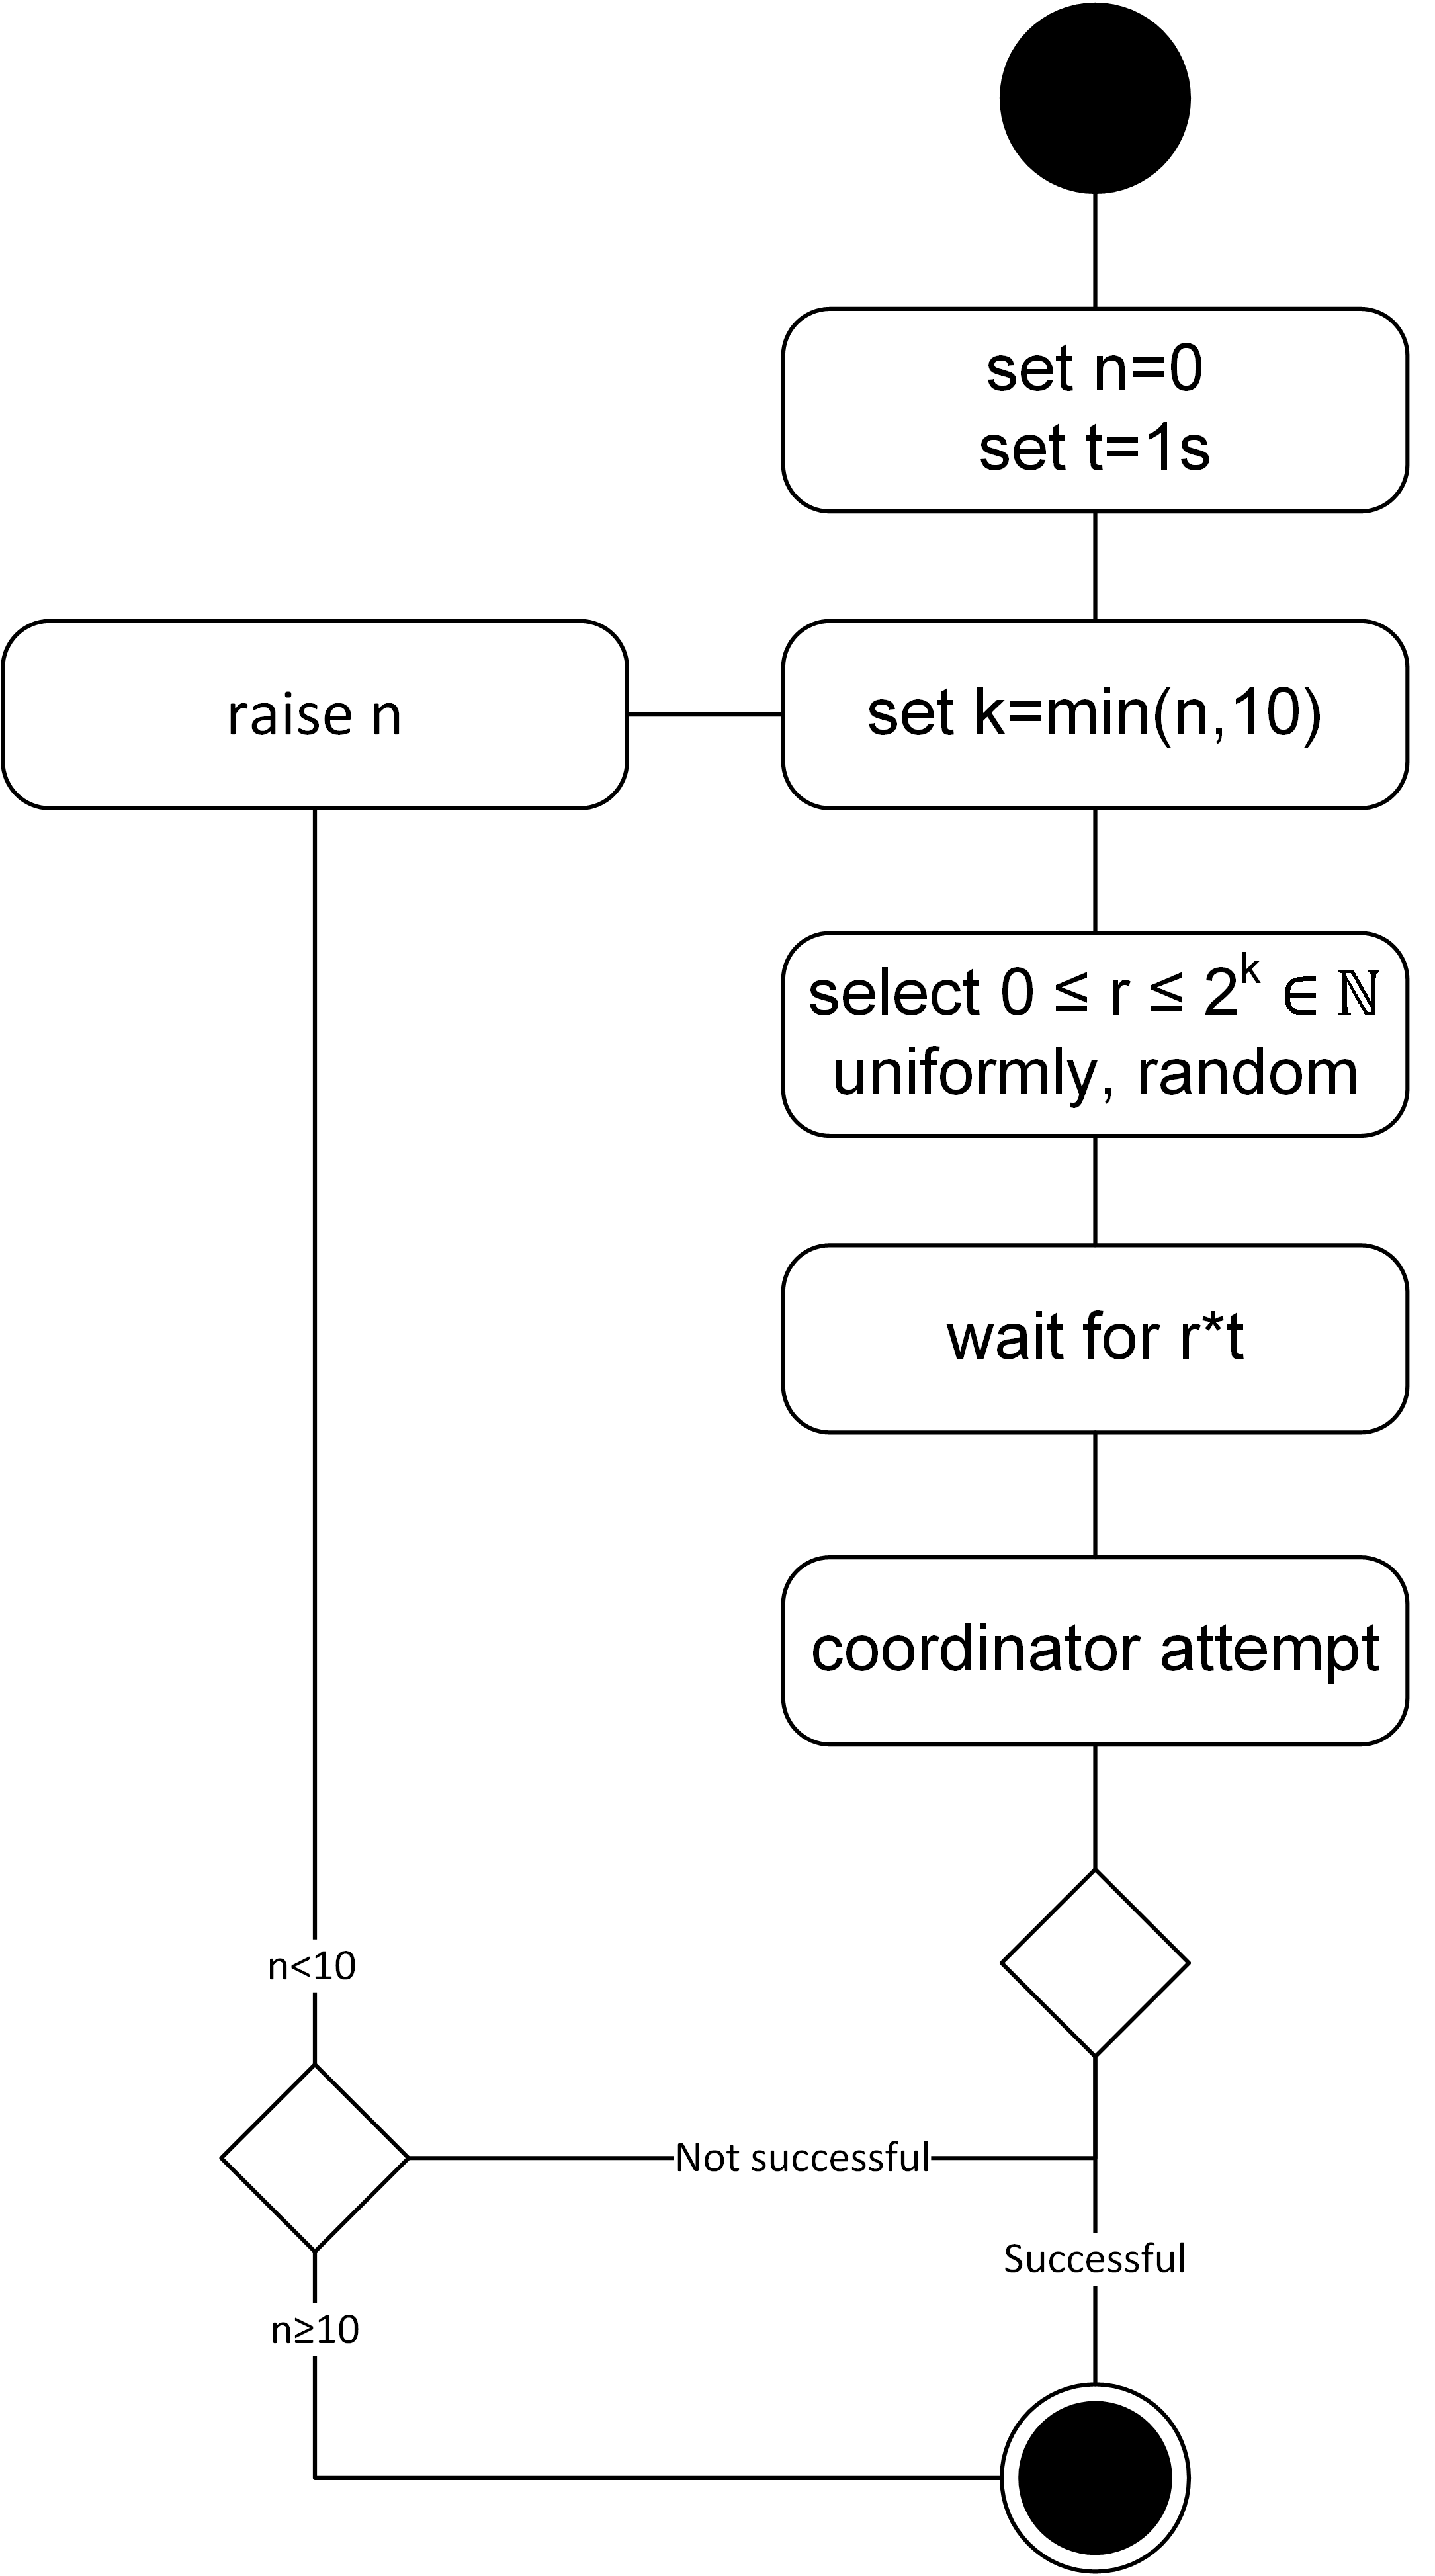
\includegraphics[scale=0.8]{figures/exponential-backoff.png}
		\label{figure:coordinator exponential backoff}
		\end{figure}
		
		\todo{heartbeat: timeout timer run out, try to send heartbeat, otherwise abort and reset initial state}
		
		\todo{Reduction of active connections; compare number of additional rounds needed; discuss timeouts}
		
		\todo{when is clock synchronization triggered? Use as transition to next action}
		
		\subsection{Clock Synchronization}
		\label{Clock synchronization}
		
		For statistical data in a gamification system, the sequence of events in infinitesimal time units is not as important as comparing the data for the same durations in \gls{UTC}, so a synchronization of physical clocks is needed. In this thesis  the well known Berkeley-algorithm for internal clock synchronization in distributed systems is used as described in \textcite{Ghosh2015}.
		
		\noindent The coordinator
		\vspace{-\topsep}
		\begin{enumerate}
			\itemsep-0.5em
			\item requests the current time values $t_i$ from participating nearby nodes $i$.
			\item computes the average of these values $t_{average}$.
			\item reports back the adjustments $\Delta_{i}=t_{average}-t_i$
		\end{enumerate}
	
		Since the communication between the coordinator and a node takes time, the received response is already outdated. This is compensated by observing the \gls{RTT} and using half as a correction value (compare \ref{eq:berkeley RTT}). The \gls{RTT} is herein the timespan between sending a request to a node and receiving its response (see figure \ref{figure:berkeley RTT}). By sending the adjustments $\Delta_i$ instead of the adjusted time, the receiving nodes do not need to compensate the received value with the \gls{RTT}.
		\begin{alignat}{1}
		t'_i &=t_i+\frac{RTT}{2}=t_i+\frac{t_e-t_s}{2} \label{eq:berkeley RTT}
		\end{alignat}
		
		\begin{figure}[htbp] % h for placement here
			\caption{Round Trip Time}
			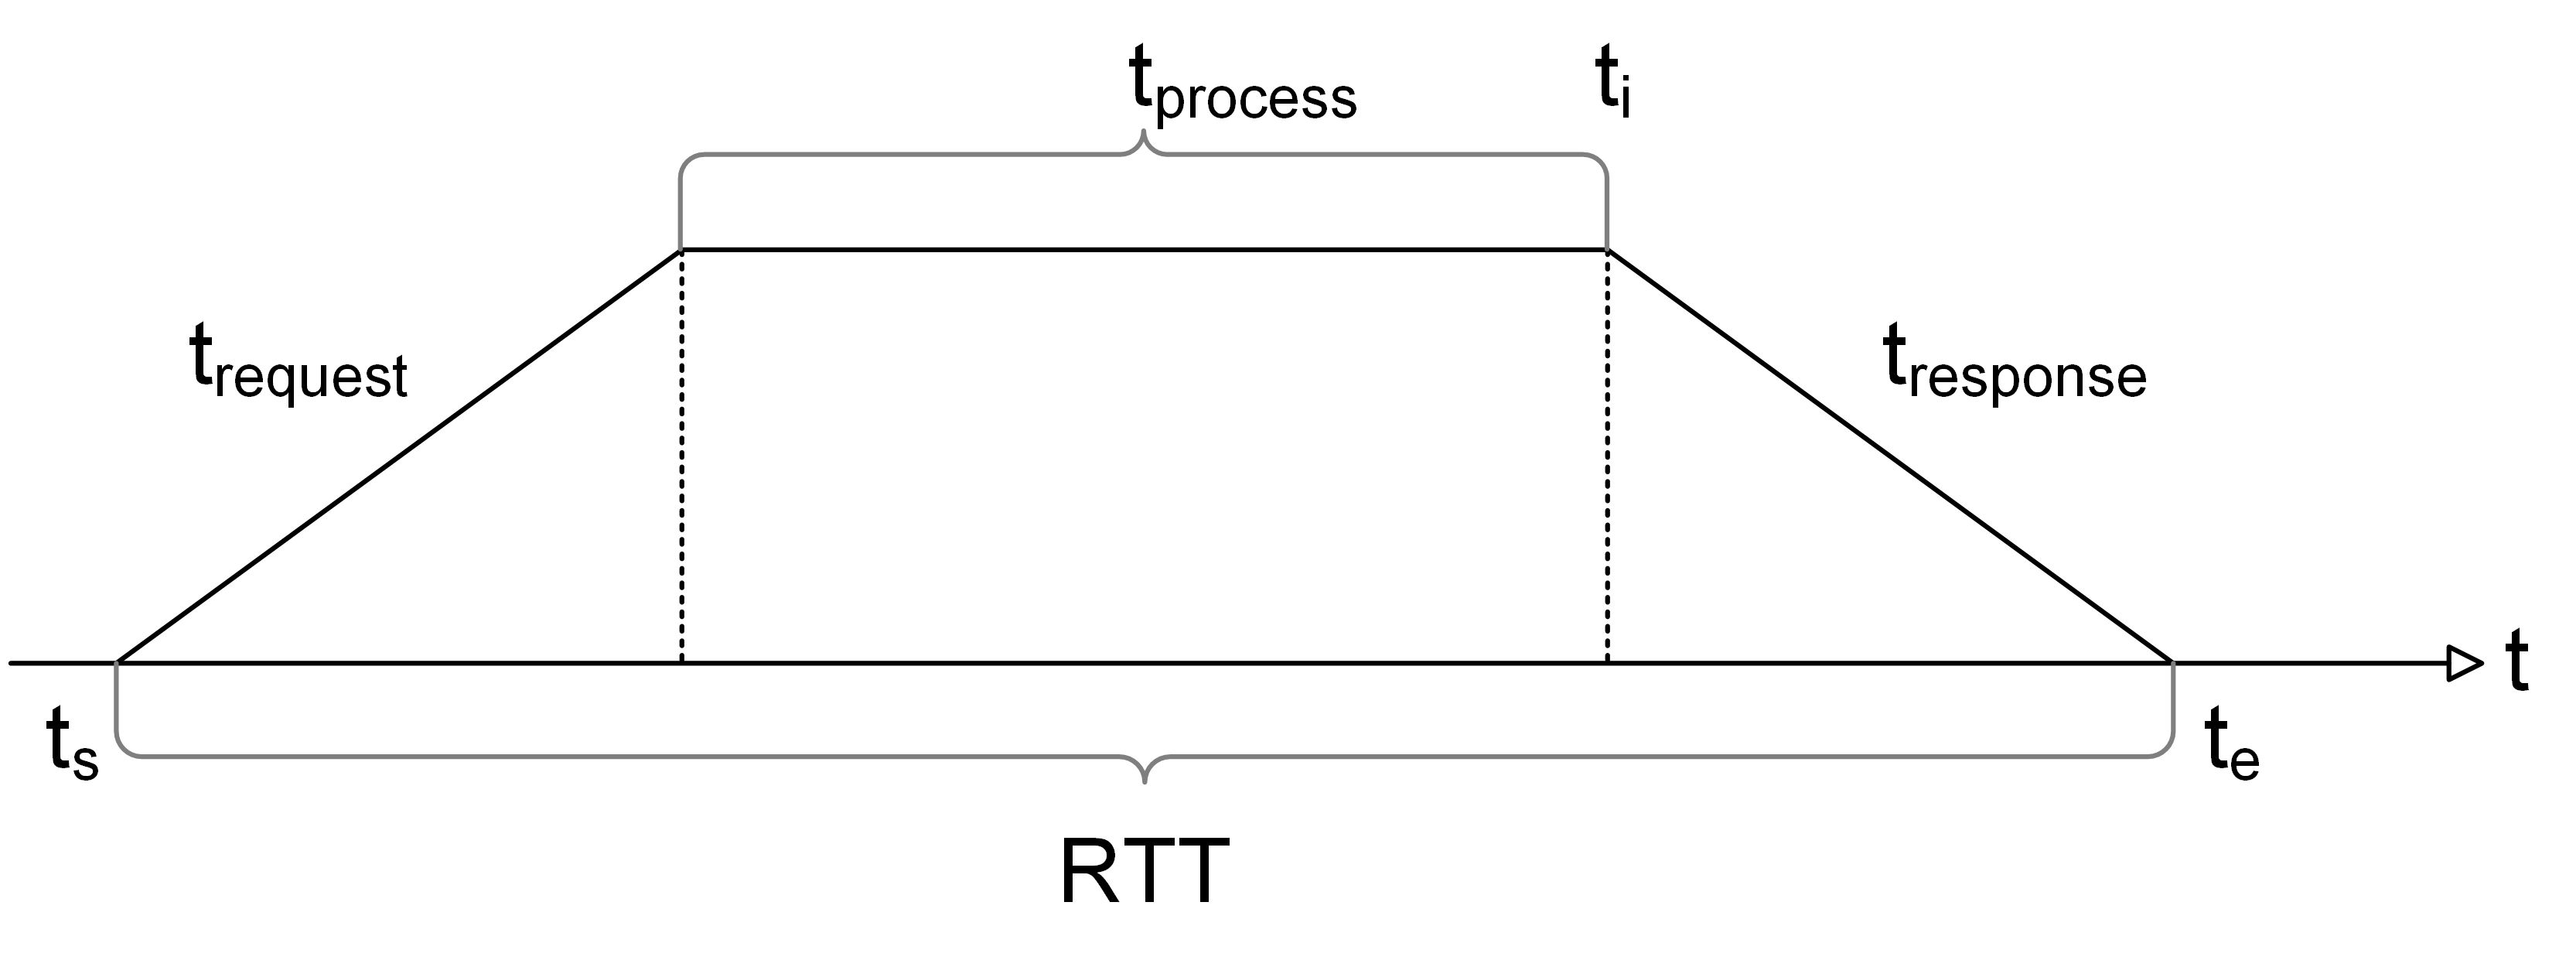
\includegraphics[scale=1.0]{figures/berkeley.png}
			\label{figure:berkeley RTT}
		\end{figure}
	
		 For further improvement of the accuracy the processing duration between receiving a request and sending the response $t_{process}$ can be measured and send to the coordinator. In this thesis the simple approximation for $t_{response}$ is used, since the additional payload extends the transmission duration (see example computation in figure \ref{figure:berkeley example}). The \gls{RTT} has to be below an upper bound though, otherwise there is to much uncertainty regarding the influence of $t_{request}$, $t_{process}$ and $t_{response}$.
		 Also bounds for the deviation of the time can be defined to reduce the influence of outliers.
		 
		 \begin{figure}[htbp] % h for placement here
		 \caption{Example computation of adjustments with Berkeley}
		 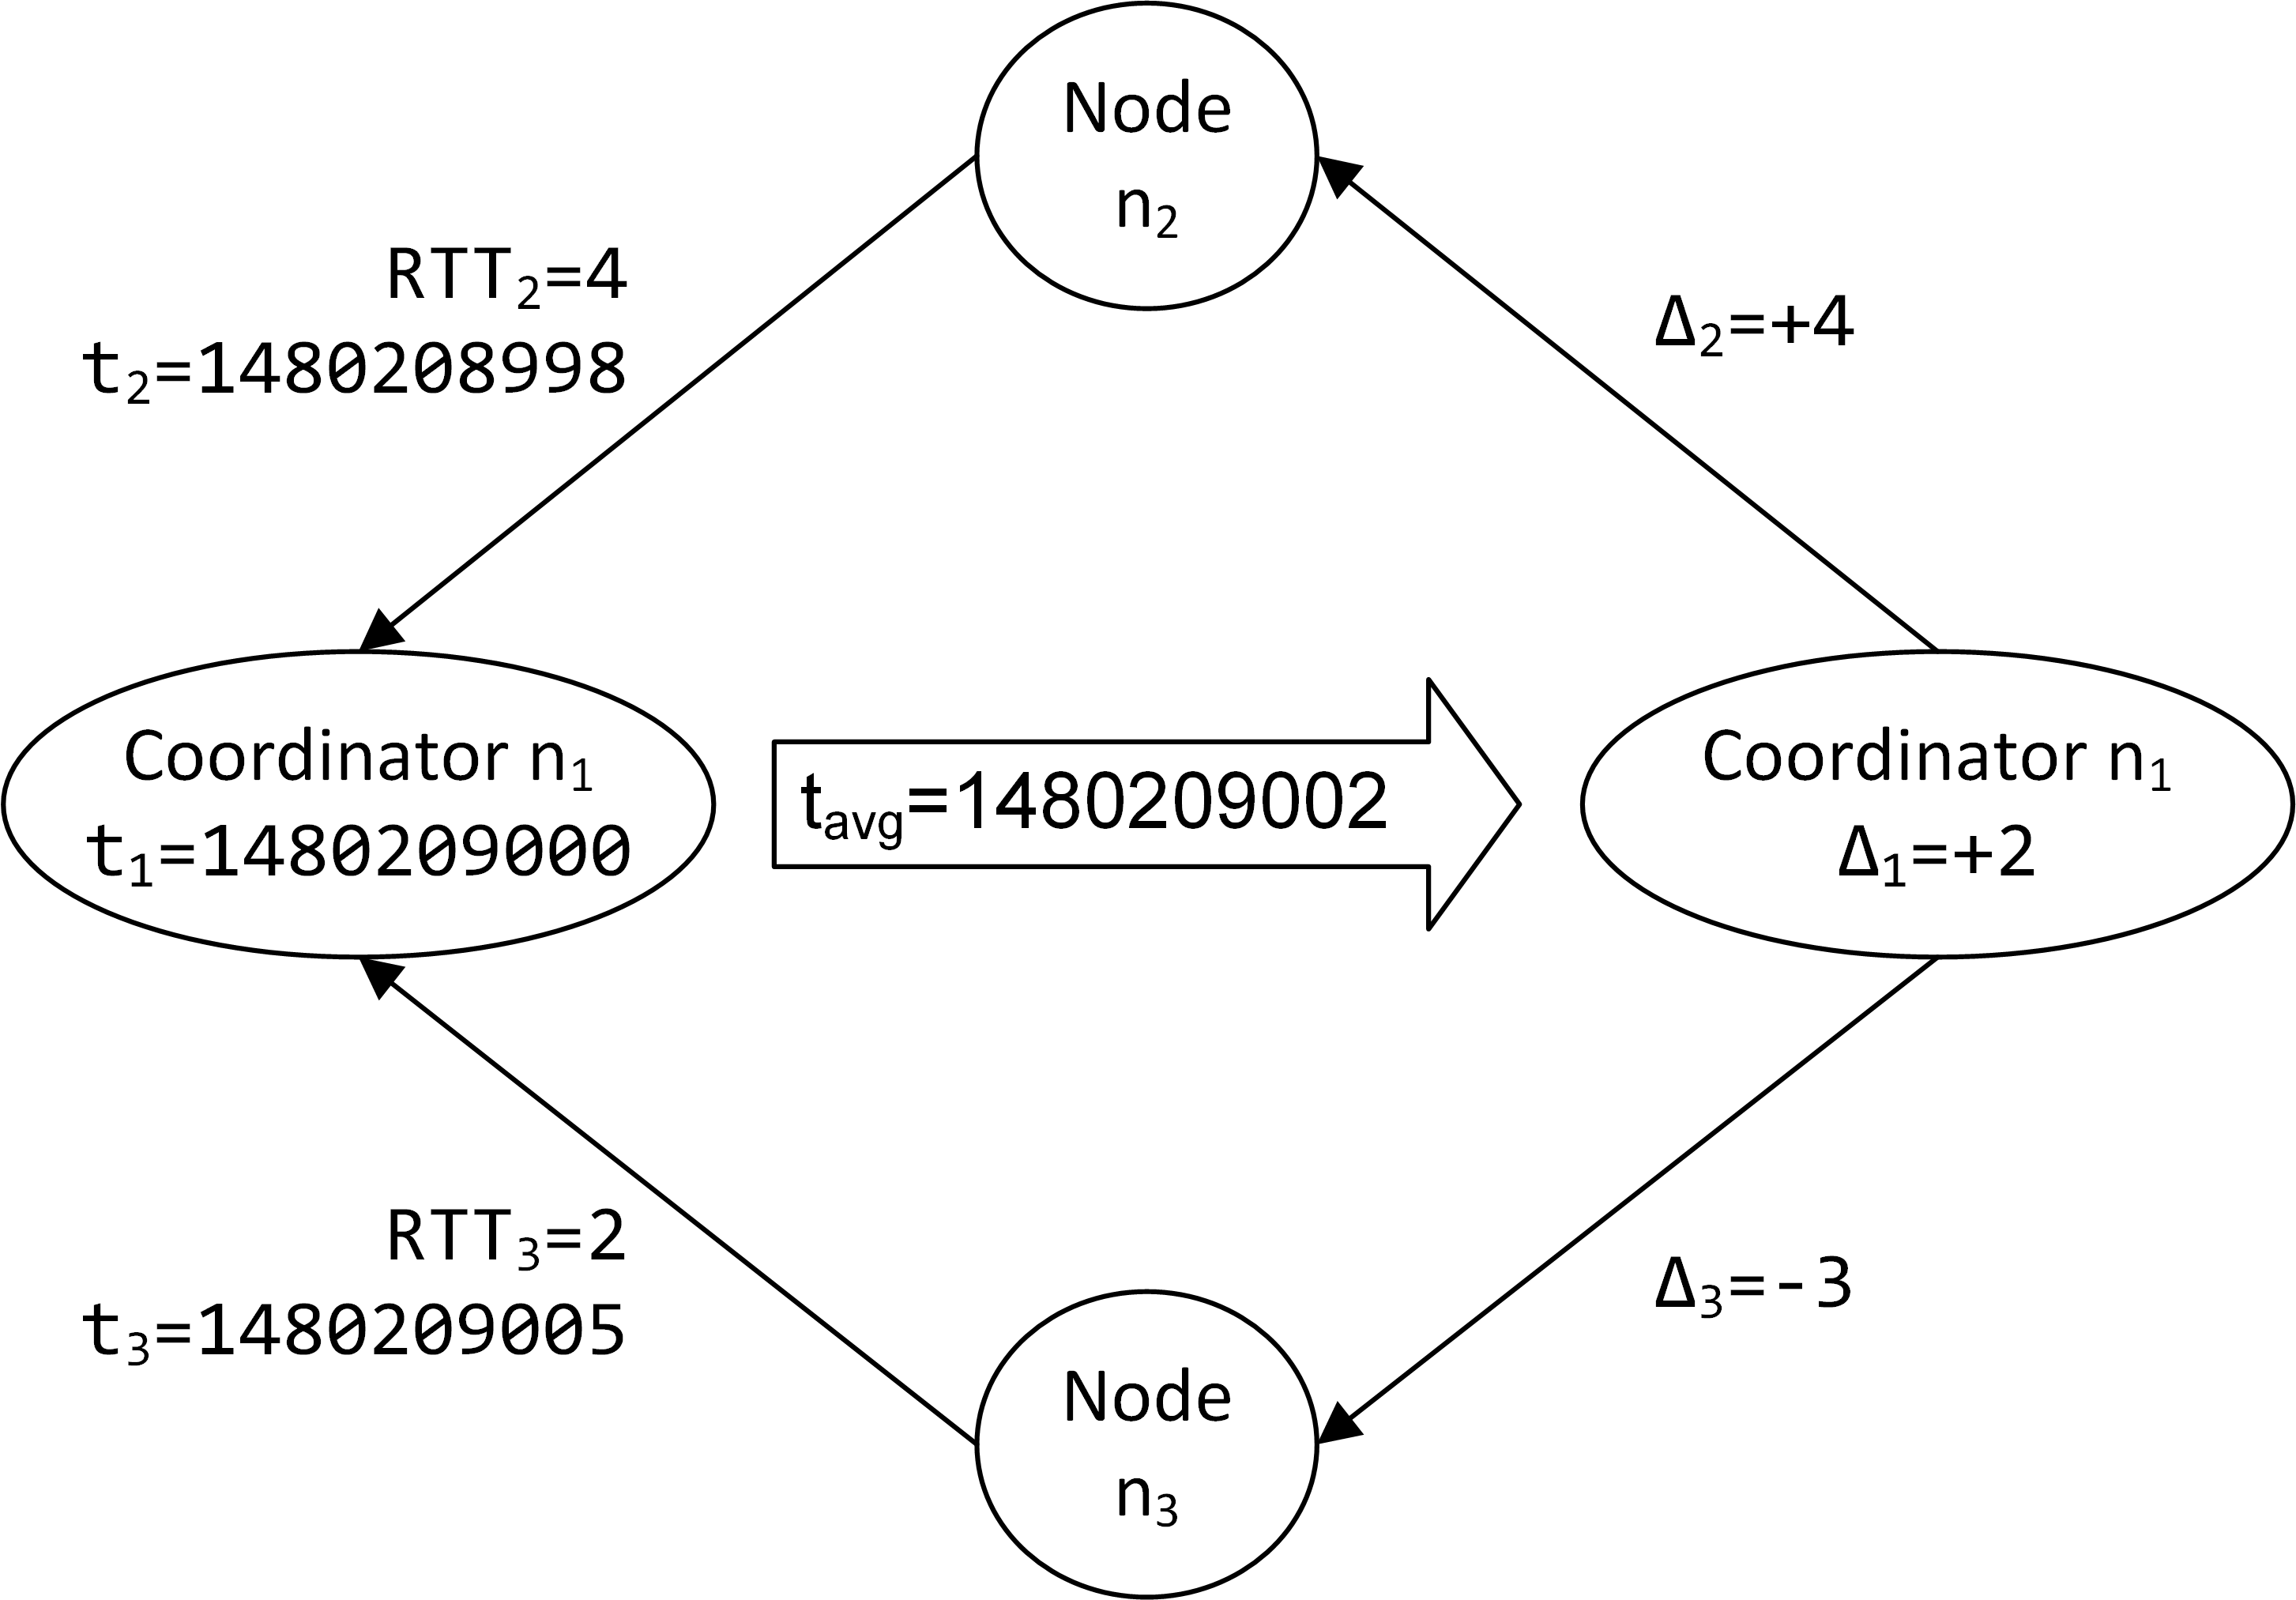
\includegraphics[scale=1.0]{figures/berkeley-example.png}
		 \label{figure:berkeley example}
		 \end{figure}
		
		\subsection{Distributed Databases}
		\label{Distributed Database}
		
		\todo{simplified version; let system handle storage; system needs to provide callback to run query over hashes; hash for each entry and db hash over all hashes; calculation done in lib; if db hash different from neighbor: compare entries anti chronologically}
		
		\todo{information: hash | time-stamp | number of participants | min v max v sum | value }
		
%	\section{Applicability of \gls{SMPC} Protocols in \gls{MANET}s} \todo{Remove Applicability chapter? More or less answered in previous/following chapters...}
	
%		\subsection*{Analysis of Key Factors: Computing Power, Network Data Rates and Duration of Connection}
		
%		\subsection*{Effectiveness of \gls{SMPC} Protocols in Sparse Networks}
		
%			\subsubsection*{Maintaining anonymity}
		
%			\subsubsection*{Strategies for Aggregation of Participants in Sparse Networks}
			
	\section{Architecture}
	\label{Architecture}
	
			% Grobdesign, Komponentenbeschreibung, globale Eigenschaft des Gesamtsystems
	
			\todo{FURPS: Functionality, Usability, Reliability, Performance, Supportability; how followed to be system independent}
	
			\todo{UML; module structure}
			
			\todo{state machine; state pattern; client server architecture; \gls{UML} state diagrams for 1. joining network (get time; set clock delta), 2. finding computation partners, 3. running computation, 4. compare database}
			
			\todo{describe how it will change for a real \gls{MANET}: simplification, reduction of states}
			
			\todo{describe what is handled internally and what is handled externally by the hosting system and why (external: providing time, providing secure seed, providing timeout timer, providing communication channel: send (id based), receive (id based), query neighbors; )}

\chapter{Implementation \todo{15-20\%; details on the implementation; for someone who wants to continue the work}}	
\label{Implementation}

	%\section{Development Tools}
	\todo{UML class or component diagram}
	
	\section{Communication Layer}
	\label{Communication Layer}
	
			\todo{UML communication diagram}
	
			\subsection{Pairing-less Connection}
			\label{Pairing-less Connection}
			
			\todo{external system: extend on \gls{RFCOMM}; widespread}
			
			\subsection{Securing Channel}
			\label{Secure Channel}
			
			\todo{describe how external system can provide better seeds for the public key system}
			
			\todo{describe how the library encrypts the messages; flag for message to signal encryption (first Byte of payload 0/1)}
			
			\todo{https://developer.android.com/reference/java/security/SecureRandom.html}
			
	\section{Secure Multi-Party Computation Module}
	\label{Secure Multi-Part Computation Module}
	
	\todo{describe the module for creating shares; describe generation of communication partner matrix; describe secure addition module; describe secure maximum module; describe secure minimum module}
	
	\section{Data Storage and Distribution}
	\label{Data Storage and Distribution}
	
	\todo{describe hash module; }
	
	\section{Interfacing the Library}
	\label{Interfacing the Library}
	
		\subsection{Configuration}
		\label{Configuration}
		
		\todo{describe configuration.h: what can be configured, override of illegal configurations/sanity checks}
		
		\subsection{Usage in C}
		\label{Usage in C}
		
		\todo{describe library is used in raspberry and in xadow}
		
		\subsection{Usage in Android}
		\label{Usage in Android}
		
		\todo{describe how library is used with android \gls{NDK}; describe Java wrapper}
		
\chapter{Evaluation \todo{5-15\%; outcome; how was it tested; for supervisor}}
\label{Evaluation}

	\section{Testing Tools}
	\label{Testing Tools}
	
		\todo{Unity (Unit test for C); JUnit; Android based multi-device tests}
		
		\todo{centralized client-server test application for android: trigger test runs, report results (measured execution time, correctness)}

	\section{Examination of Computation Time Dependent on Computing Power}
	\label{Examination of Computation Time Dependent on Computing Power}
	
	\todo{test on: xadow (IoT); RaspberryPi 3 (SBC); Android 4 (single core, low RAM), Android 5 (multi-core, 2 GB RAM)}
	
	\section{Examination of Computation Time Dependent on Number of Participants}
	\label{Examination of Computation Time Dependent on Number of Participants}
		
		\todo{n devices, n shares (highest security)}
		
		\todo{n devices, k (>n/2) shares (adjustable security)}
			
		%\todo{SNET with increasing number of android devices; predefined tests}
		
		%\section{Examination of Distribution Time Dependent on Number of Participants}

\chapter{Discussion \todo{5-15\%; outcome for a design-reader} }
\label{Discussion}

\todo{extend protocol: implement merging of results, to reduce probability of not finding computation partner; implement alternative protocols}

\todo{implement optional verification for addition, if performance is good enough for real life application}

\chapter{Conclusion \todo{5-10\%; outcome for an introduction-reader}}
\label{Conclusion}

\todo{outlook: bt 5.0, mesh network}

\clearpage
\renewcommand{\bibname}{References} % rename Bibliograpy to References
\printbibliography[heading=bibintoc] % add References chapter and display it in toc

\begin{appendices}
	\chapter{Some name}
	\lipsum[3]
\end{appendices}

\end{document}